\subsection{Q1: Exploration 2.6.1 (Page 49)}
\label{Q1:Expl 2.6.1 SubSection}

\subsubsection{Task 2.1}
\label{Q1:Expl 2.6.1(2.1) SubSubSection}

\begin{tcolorbox}[colback=gray!20!white,colframe=gray!20!white]
  \emph{\textbf{Question 2.1 (a)} Describe the effects on the neural response of increasing $g_{bar\_e}$ to .5, and of decreasing it to .3. \textbf{(b)} Is there a qualitative difference in the unit activation (act) between these two changes of magnitude .1 away from the initial .4 value? \textbf{(c)} What important aspect of the point neuron activation function does this reveal? [Mark: 11]} 
\end{tcolorbox} 
\vspace{0.5cm}

When increasing the value of the excitatory conductance ($g_{bar\_e}$) from 0.4 to 0.5, the value of the activation value for a neural response (receiving unit) increases from 0.7204 to 0.9445 as showing in \cref{Q2.1 - 0.4} and \cref{Q2.1 - 0.5} and indicating a relationship between the excitatory conductance ($g_{bar\_e}$) and the receiving unit. When changing $g_{bar\_e}$ from 0.4/0.5 to 0.3, the neural response is null as seen in \cref{Q2.1 - 0.3}, where the receiving unit doesn't pick up any value despite the sending unit ($g_{bar\_i}$) remaining the same. When comparing the graphical output data shown in \cref{Q2.1 - 0.4G}, \cref{Q2.1 - 0.5G} and \cref{Q2.1 - 0.3G} for the 3 values of $g_{bar\_e}$ (0.4, 0.5 and 0.3 respectively). The activation value stems from the membrane potential ($V_m$), which for all 3 graphs shows a 0.2241 increase for $g_{bar\_e}$ at 0.4 to 0.5, Ultimately when $g_{bar\_e}$ equals 0.3 then the activation value flat lines in \cref{Q2.1 - 0.3G} as it return a null value. This highlights how the point neuron activation function relates to the input excitatory conductance directly affects the total activation value.

\newpage
\begin{multicols}{2}
\begin{figure}[H]
\centering
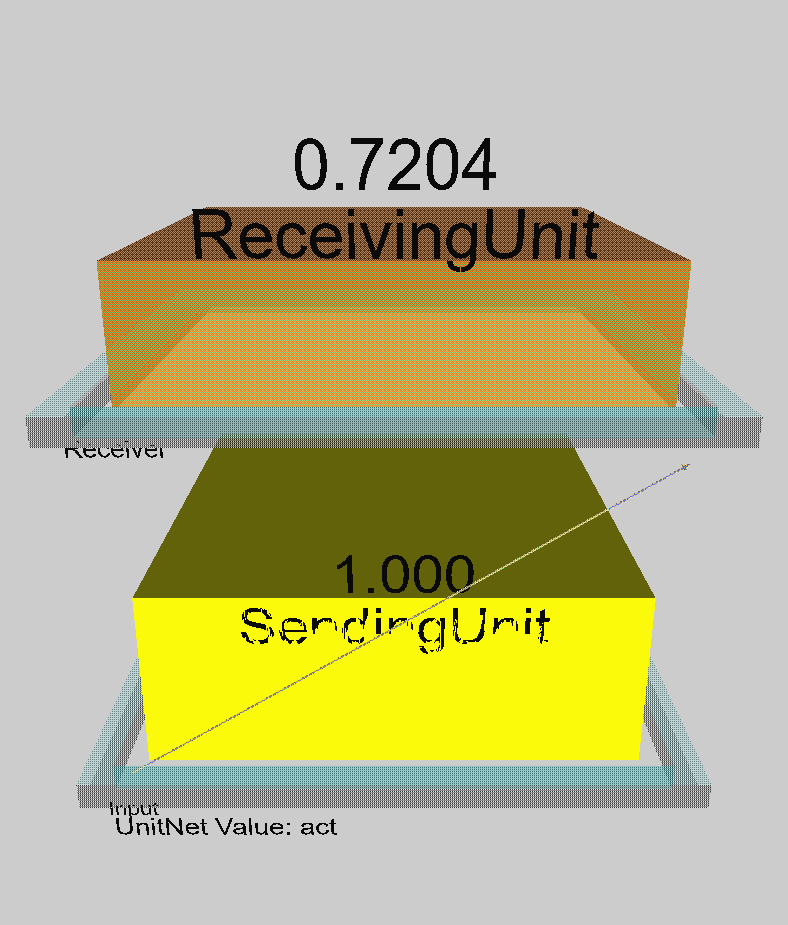
\includegraphics[scale=0.225]{Media/Main/EQ1/2.1.A.png}
\caption{Visual representation of the sending and receiving units with $g_{bar\_e}$.}
\label{Q2.1 - 0.4}
\end{figure}

\begin{figure}[H]
\centering
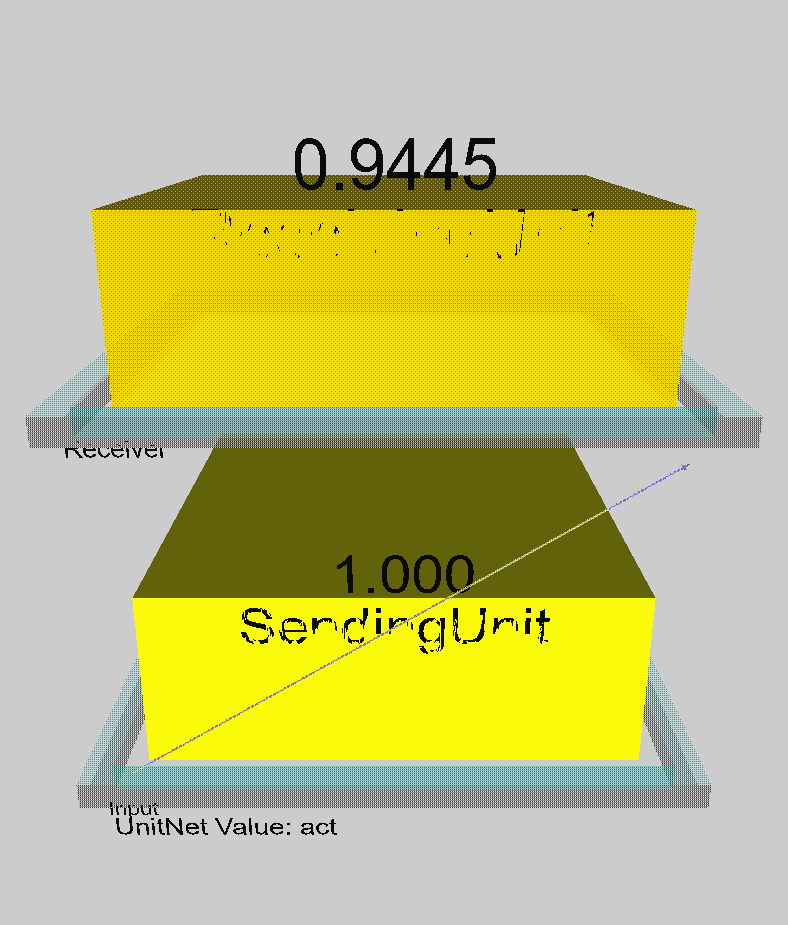
\includegraphics[scale=0.225]{Media/Main/EQ1/2.1.Aa.png}
\caption{Visual representation of the sending and receiving units with $g_{bar\_e}$.}
\label{Q2.1 - 0.5}
\end{figure}

\begin{figure}[H]
\centering
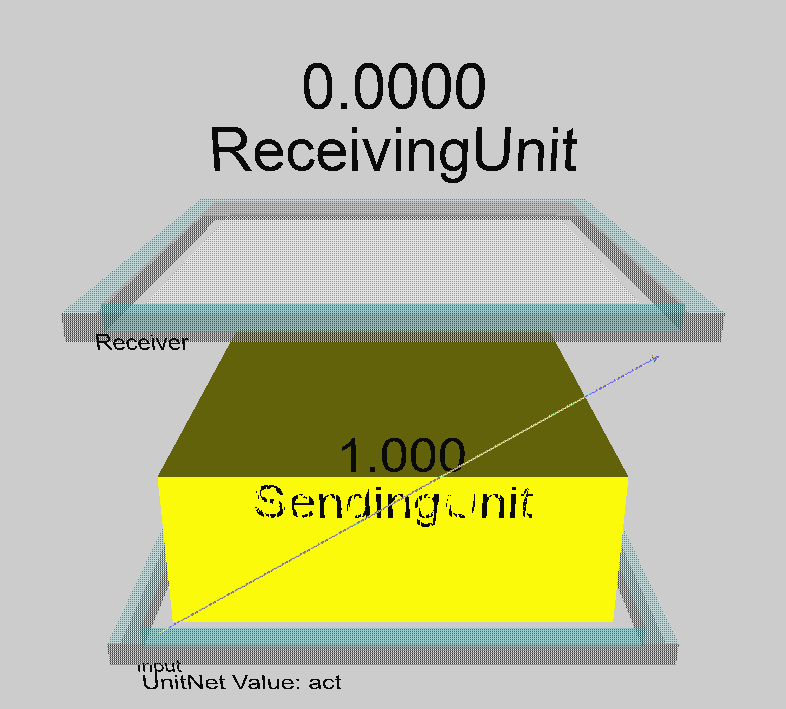
\includegraphics[scale=0.225]{Media/Main/EQ1/2.1.Ab.png}
\caption{Visual representation of the sending and receiving units with $g_{bar\_e}$.}
\label{Q2.1 - 0.3}
\end{figure}

\begin{figure}[H]
\centering
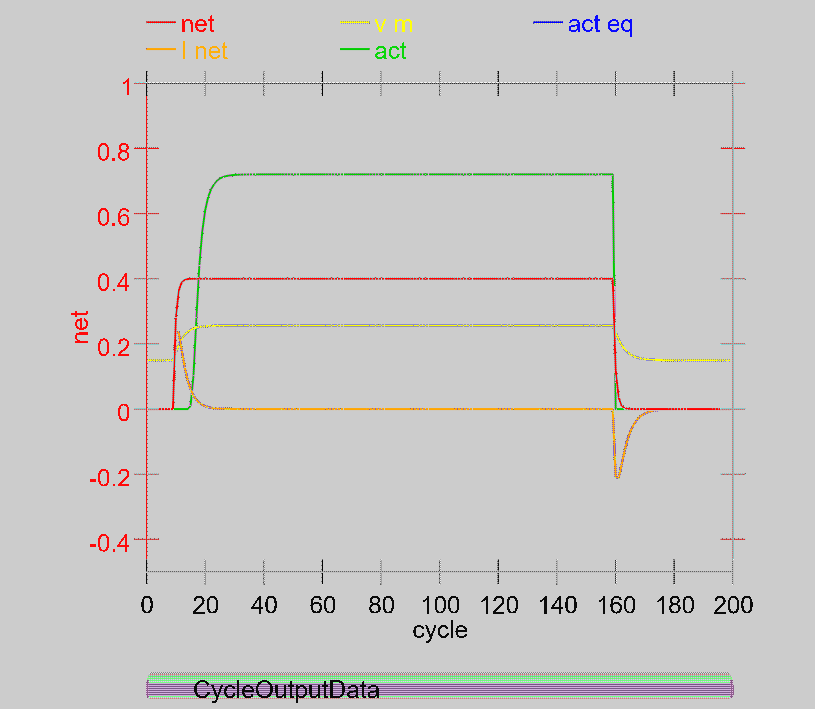
\includegraphics[scale=0.3]{Media/Main/EQ1/2.1.AG.png}
\caption{Graphical output data of \cref{Q2.1 - 0.4} when running a value of 0.4 for $g_{bar\_e}$.}
\label{Q2.1 - 0.4G}
\end{figure}

\begin{figure}[H]
\centering
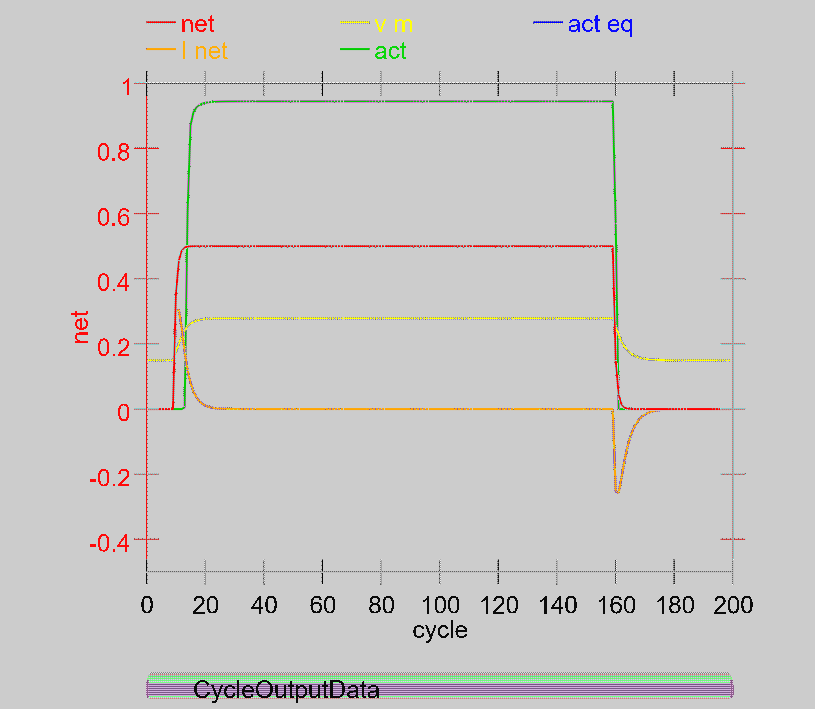
\includegraphics[scale=0.3]{Media/Main/EQ1/2.1.AaG.png}
\caption{Graphical output data of \cref{Q2.1 - 0.5} when running a value of 0.5 for $g_{bar\_e}$.}
\label{Q2.1 - 0.5G}
\end{figure}

\begin{figure}[H]
\centering
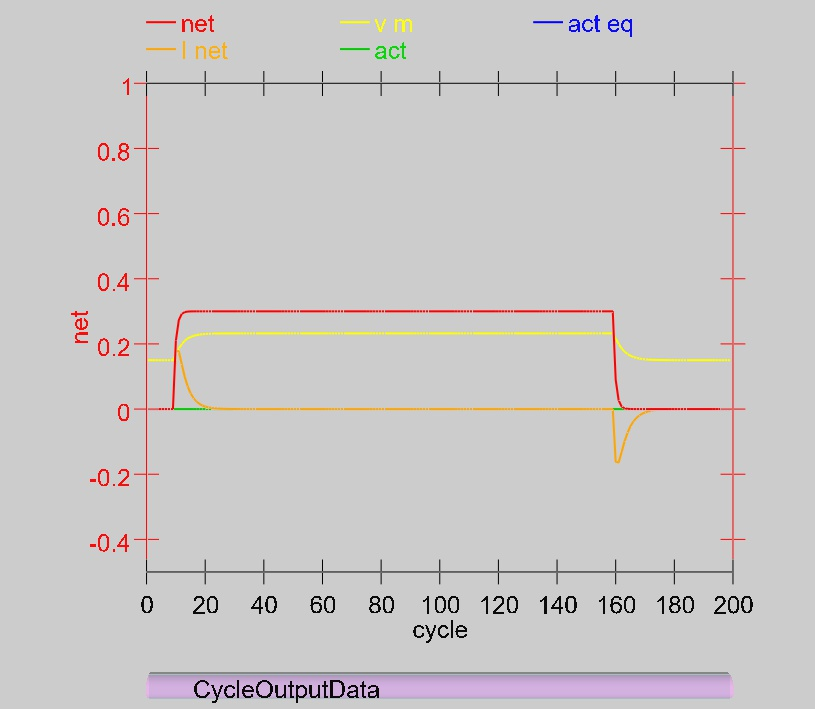
\includegraphics[scale=0.3]{Media/Main/EQ1/2.1.AbG.png}
\caption{Graphical output data of \cref{Q2.1 - 0.3} when running a value of 0.3 for $g_{bar\_e}$.}
\label{Q2.1 - 0.3G}
\end{figure}
\end{multicols}


\subsubsection{Task 2.2}
\label{Q1:Expl 2.6.1(2.2) SubSubSection}

\begin{tcolorbox}[colback=gray!20!white,colframe=gray!20!white]
  \emph{\textbf{Question 2.2 (a)} To 3 decimal places, what value of $g_{bar\_e}$ puts the unit just over threshold? Can you think of a better way of finding this value (Hint: Do you remember an equation for the equilibrium membrane potential given a particular set of inputs?) \textbf{(b)} Compute the exact value of excitatory input required to just reach threshold, showing your math (note that: $g_l$ is always 1 because the leak channels are always open; $g_e$ is 1 when the input is on; inhibition is not present here and can be ignored). Does this agree with your empirically determined value? \textbf{(Hint: It should!)} [Mark: 8]}
\end{tcolorbox} 
\vspace{0.5cm}

By experimenting with different values for $g_{bar\_e}$ less than 0.4 to determine the threshold of the receiving unit where its value is limited to 0.0001 at a minimum $g_{bar\_e}$ value of 0.324 (restricted to 3 decimal places). By using the equilibrium membrane potential equation, the minimum value of $g_{bar\_e}$ can be calculated to which reaches threshold of the neural response. \\

\textbf{Equilibrium Membrane Potential Equation:}
\begin{equation}
0 = g_e(t) \bar{g_e} (E_e - V_m(t))+ g_i(t) \bar{g_i} (E_i - V_m(t)) + g_l(t) \bar{g_l} (E_l - V_m(t))
\label{Equil Memb Pot Eq}
\end{equation}

\textbf{Re-Written As:}
\begin{equation}
V_m = \dfrac{g_e \bar{g_e}}{g_e \bar{g_e} + g_i \bar{g_i} + g_l \bar{g_l}} E_e + \dfrac{g_e \bar{g_e}}{g_e \bar{g_e} + g_i \bar{g_i} + g_l \bar{g_l}} E_i + \dfrac{g_e \bar{g_e}}{g_e \bar{g_e} + g_i \bar{g_i} + g_l \bar{g_l}} E_l
\label{New Equil Memb Pot Eq}
\end{equation}

\textbf{Alternative Formulation:}
\begin{equation}
V_m = \dfrac{g_e \bar{g_e} E_e + g_i \bar{g_i} E_i + 1 \bar{g_l} E_l}{g_e \bar{g_e} + g_i \bar{g_i} + g_l \bar{g_l}}
\label{Alt Equil Memb Pot Eq}
\end{equation}

\textbf{Excitatory Input Calculation:}
\begin{equation}
V_m = \dfrac{g_e \bar{g_e} E_e + g_l \bar{g_l} E_l}{g_e \bar{g_e} + g_l \bar{g_l}} \rightarrow \dfrac{g_e \bar{g_e} E_e + 1 \bar{1} E_l}{g_e \bar{g_e} + 1 \bar{1}} \rightarrow \dfrac{g_e \bar{g_e} E_e + E_l}{g_e \bar{g_e} + 1} 
\label{Q2.2 Calculation}
\end{equation}

\begin{equation}
\dfrac{g_e \bar{g_e} E_e}{g_e \bar{g_e}} = V_m - \dfrac{E_l}{1} \rightarrow V_m - E_l
\label{Q2.21 Calculation}
\end{equation}

\begin{equation}
E_e = V_m - E_l
\label{Q2.22 Calculation}
\end{equation}

\subsubsection{Task 2.3}
\label{Q1:Expl 2.6.1(2.3) SubSubSection}

\begin{tcolorbox}[colback=gray!20!white,colframe=gray!20!white]
  \emph{\textbf{Question 2.3 (a)} How does the response of the unit change when you change $g_{bar\_l}$? Why? \textbf{(b)} How does this differ from changes to $g_{bar\_e}$? \textbf{(c)} Use the same technique you used in the previous question to compute the exact amount of leak current necessary to put the membrane potential exactly at threshold when the $g_{bar\_e}$ value is at the default of .4 (show your math). [Mark: 11]}
\end{tcolorbox} 
\vspace{0.5cm}

The original input values are graphical plotted in \cref{Q2.30} to provide a reference when changing the value of $g_{bar\_l}$. The reference value of $g_{bar\_l}$ is 2.8, where all other variables are set in \cref{Q2.3 Table} and the comparing all the graphical plots, it's clear to see that the activation value of the receiving unit increasing when the original value of $g_{bar\_l}$ is decreased, then vice versa where the activation value decreases when $g_{bar\_l}$ is increased. When changing $g_{bar\_e}$, the net input is changed whereas the activation value changes as well, where when increasing $g_{bar\_e}$, the activation value increases as well and as it decreases, the activation value decreases also. However in the case of $g_{bar\_l}$ as it increases the value of the activation value decreases, the opposite of what happens with $g_{bar\_e}$. \\ 


\begin{table}[H]
\begin{center}
 \footnotesize
 \begin{tabular}{|c||c|c|c|c|c||c|}
 \hline
 \multicolumn{7}{|c|} {} \\
  States & $g_{bar\_e}$ & $g_{bar\_l}$ & $g_{bar\_i}$ & $g_{bar\_h}$ & $g_{bar\_a}$ & Graphical Plot\\
 \hline \hline
 0 & 0.4 & 2.8 & 1.0 & 0.1 & 0.1 & \cref{Q2.30}\\\hline
 1 & 0.4 & 3.0 & 1.0 & 0.1 & 0.1 & \cref{Q2.31} \\\hline
 2 & 0.4 & 3.2 & 1.0 & 0.1 & 0.1 & \cref{Q2.32} \\\hline
 3 & 0.4 & 2.5 & 1.0 & 0.1 & 0.1 & \cref{Q2.33} \\\hline
 4 & 0.4 & 2.2 & 1.0 & 0.1 & 0.1 & \cref{Q2.34} \\\hline
 \end{tabular} \\ 
 \caption{Tabulated results of changing $g_{bar\_l}$.}
 \label{Q2.3 Table}
\end{center}
\end{table}


\begin{figure}[H]
\centering
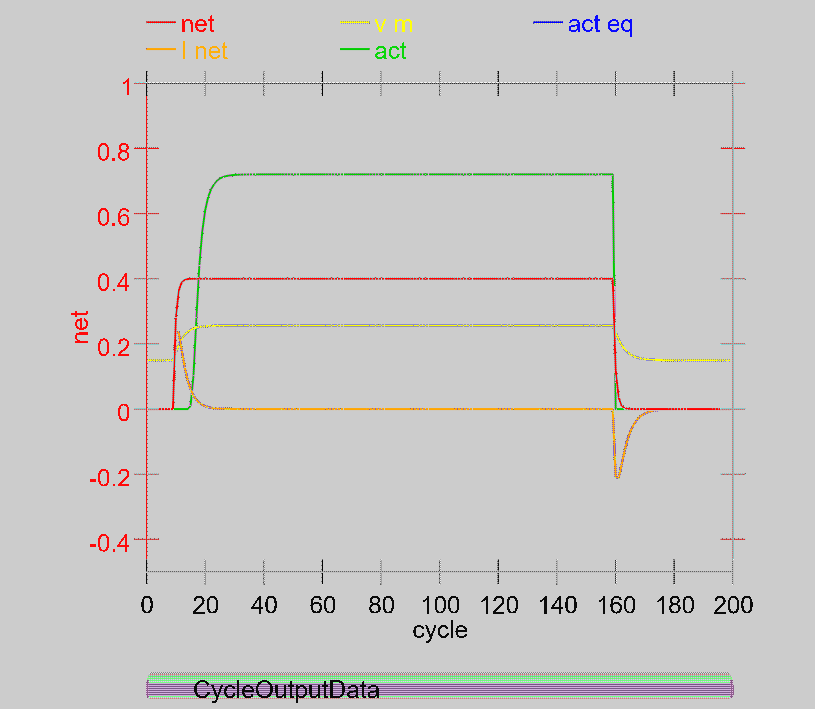
\includegraphics[scale=0.5]{Media/Main/EQ1/2.1.AG.png}
\caption{Graphical output of the system where $g_{bar\_l}$ is at the original value of 2.8.}
\label{Q2.30}
\end{figure}

\newpage

\begin{multicols}{2}
\begin{figure}[H]
\centering
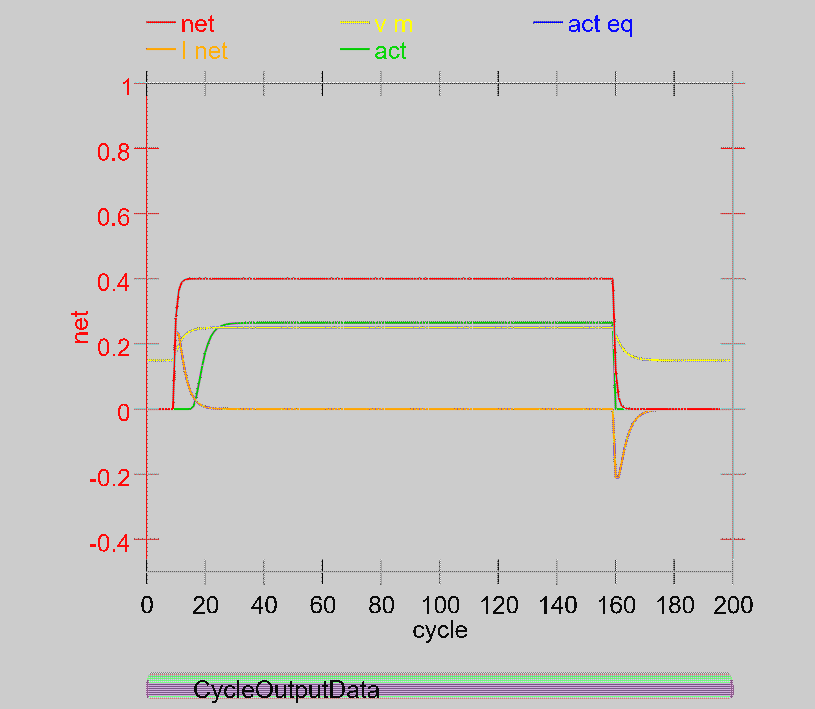
\includegraphics[scale=0.4]{Media/Main/EQ1/2.3.S1G.png}
\caption{Graphical output of the system where $g_{bar\_l}$ is at a value of 3.0.}
\label{Q2.31}
\end{figure}

\begin{figure}[H]
\centering
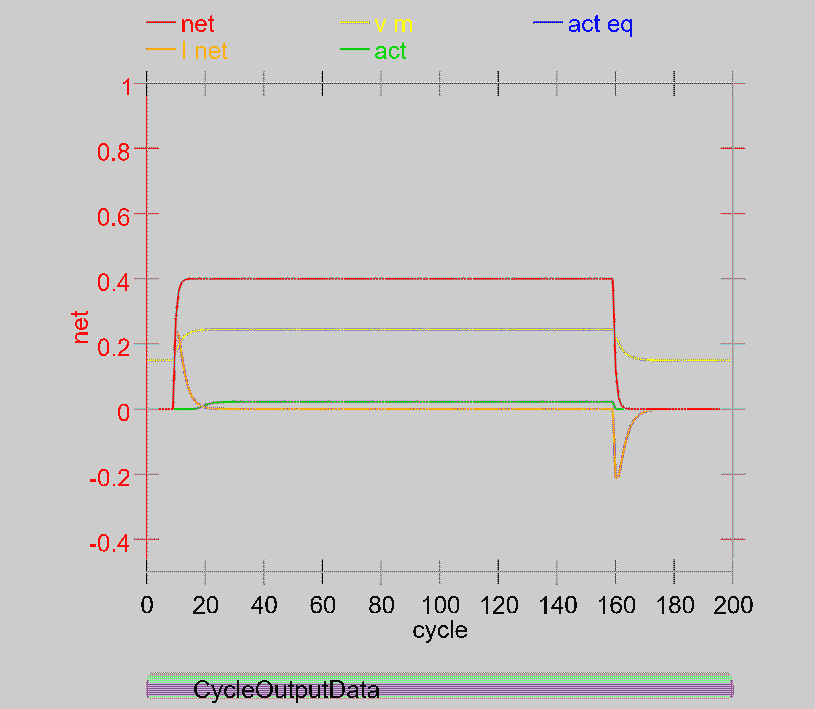
\includegraphics[scale=0.4]{Media/Main/EQ1/2.3.S2G.png}
\caption{Graphical output of the system where $g_{bar\_l}$ is at a value of 3.2.}
\label{Q2.32}
\end{figure}

\begin{figure}[H]
\centering
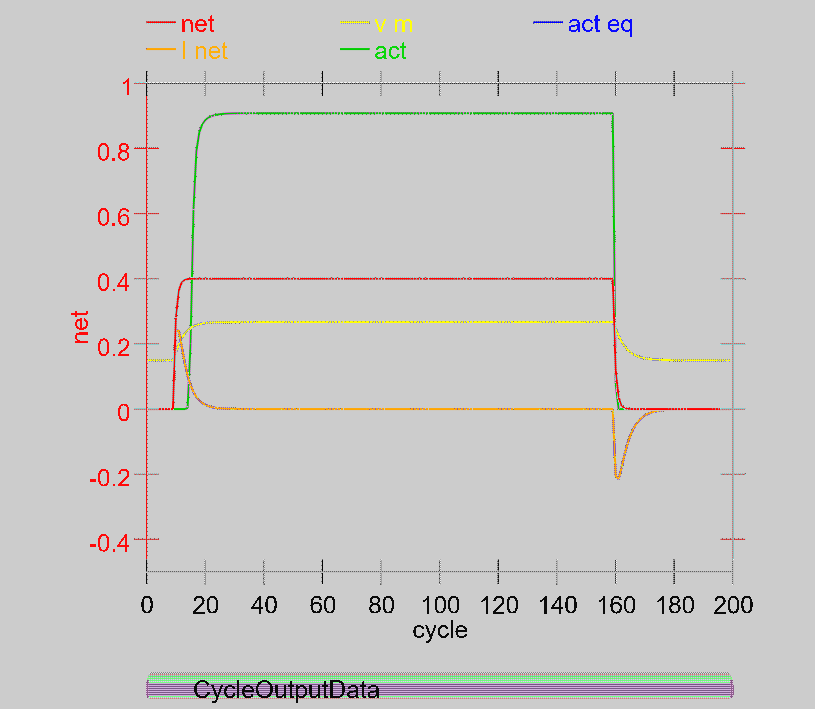
\includegraphics[scale=0.4]{Media/Main/EQ1/2.3.S3G.png}
\caption{Graphical output of the system where $g_{bar\_l}$ is at a value of 2.5.}
\label{Q2.33}
\end{figure}

\begin{figure}[H]
\centering
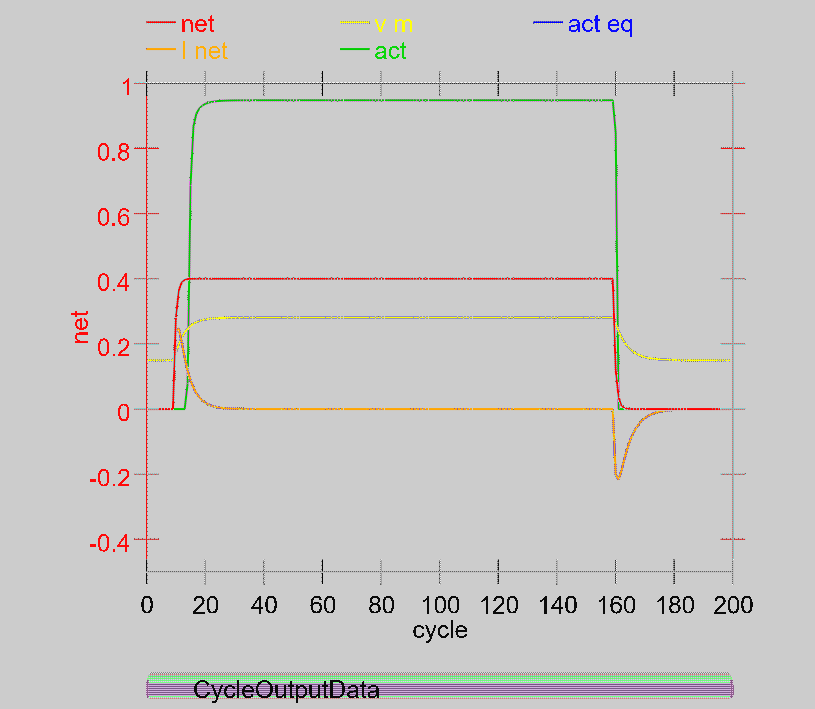
\includegraphics[scale=0.4]{Media/Main/EQ1/2.3.S4G.png}
\caption{Graphical output of the system where $g_{bar\_l}$ is at a value of 2.2.}
\label{Q2.34}
\end{figure}
\end{multicols}


\subsubsection{Task 2.4}
\label{Q1:Expl 2.6.1(2.4) SubSubSection}

\begin{tcolorbox}[colback=gray!20!white,colframe=gray!20!white]
  \emph{\textbf{Question 2.4 (a)} What happens to the unit’s activity if you change the leak reversal potential $e_{rev\_l}$ from .15 to 0? \textbf{(b)} What about when you increase it to .2? For both questions, explain the results, taking note of what happens before the input goes on as well as what happens while it is on. \textbf{(c)} What can you conclude about the relationship between the resting potential and the leak reversal potential? [Mark: 11]}
\end{tcolorbox} 
\vspace{0.5cm}

Changing the value of $e_{rev\_l}$ form 0.15 to 0 can be seen graphical in \cref{Q4.4} and \cref{Q4.5}. it can be seen when changing the leak reverse potential where the activation level equals to 0 and then when increasing it to 0.2 in \cref{Q4.6} the activation value reaches 1 in which influences the resulting membrane potential. When the $e_{rev\_l}$ is 0.2 the net current is identical to when $e_{rev\_l}$ is 0.15, this is probably due due to the small difference in value but can be seen with the rise of the activation value. However the net current starts negatives within the first 20 cycles (shown in \cref{Q4.5}) whereas when the value is positive the net current starts positive but both cases equal zero when the activation level is activated as the current is null while the activation level is reached. \\



\newpage
\begin{multicols}{2}
\begin{figure}[H]
\centering
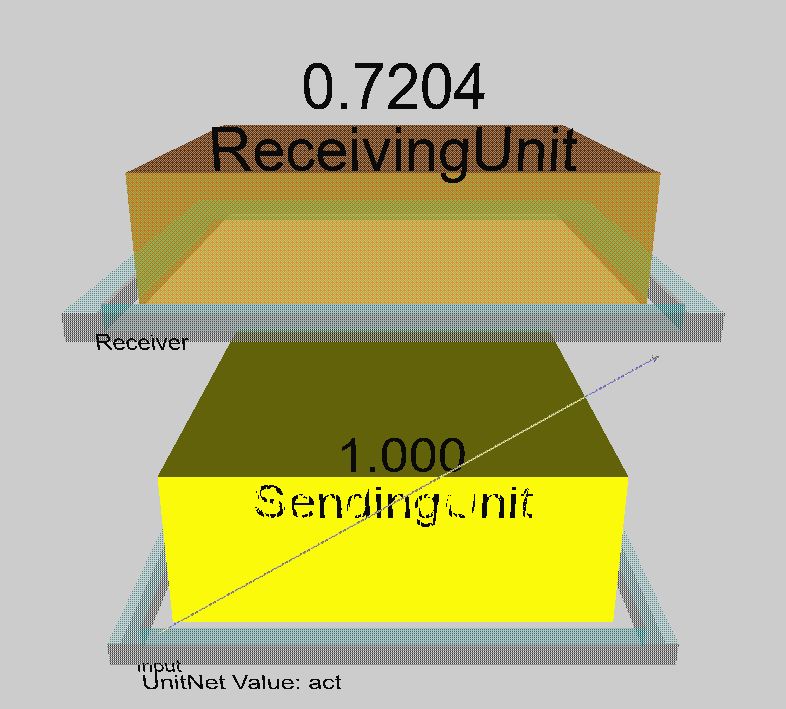
\includegraphics[scale=0.225]{Media/Main/EQ1/2.4.S0.png}
\caption{Visual representation of the sending and receiving units with $e_{rev\_l}$ at a value of 0.15.}
\label{Q4.1}
\end{figure}

\begin{figure}[H]
\centering
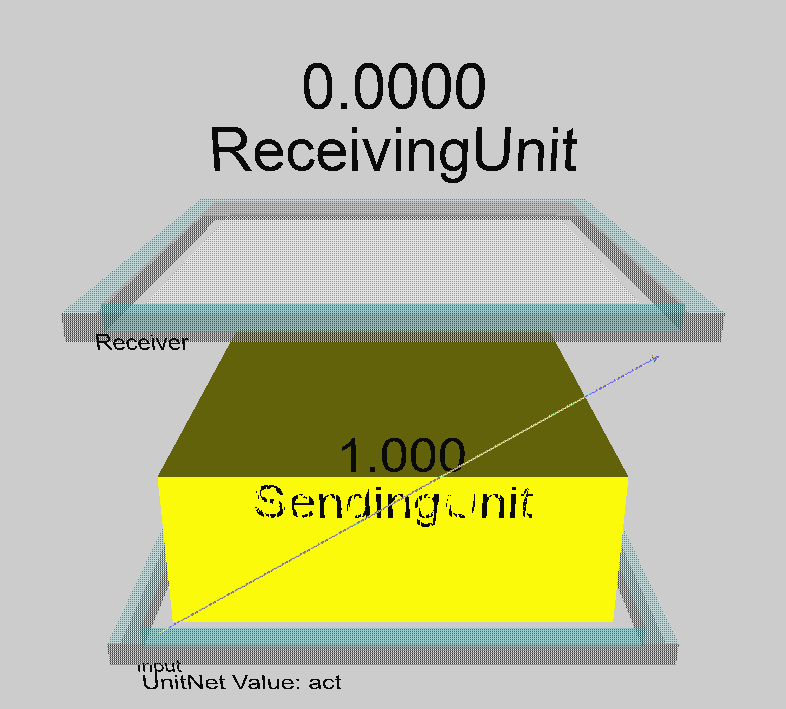
\includegraphics[scale=0.225]{Media/Main/EQ1/2.4.S1.png}
\caption{Visual representation of the sending and receiving units with $e_{rev\_l}$ at a value of 0.0.}
\label{Q4.2}
\end{figure}

\begin{figure}[H]
\centering
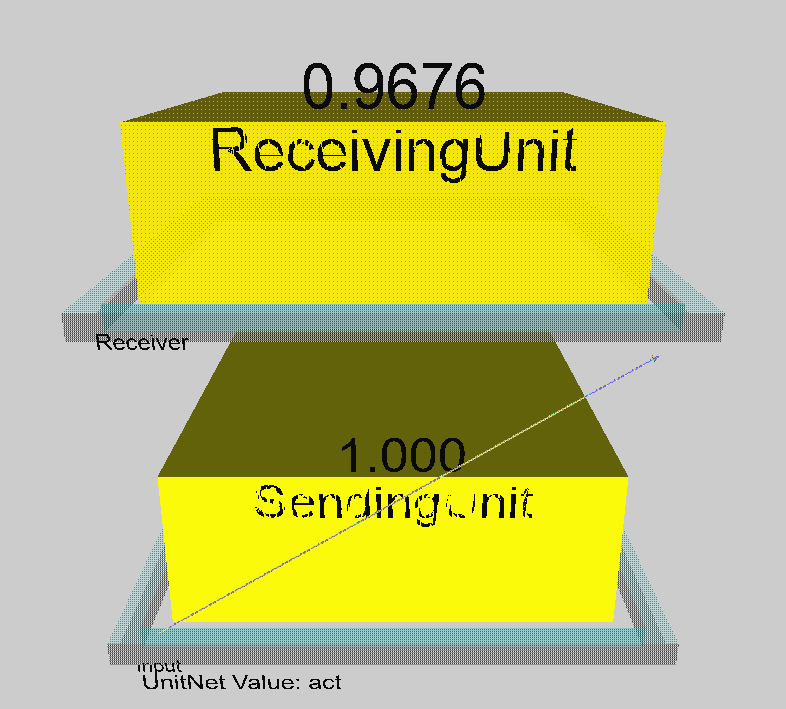
\includegraphics[scale=0.225]{Media/Main/EQ1/2.4.S2.png}
\caption{Visual representation of the sending and receiving units with $e_{rev\_l}$ at a value of 0.2.}
\label{Q4.3}
\end{figure}

\begin{figure}[H]
\centering
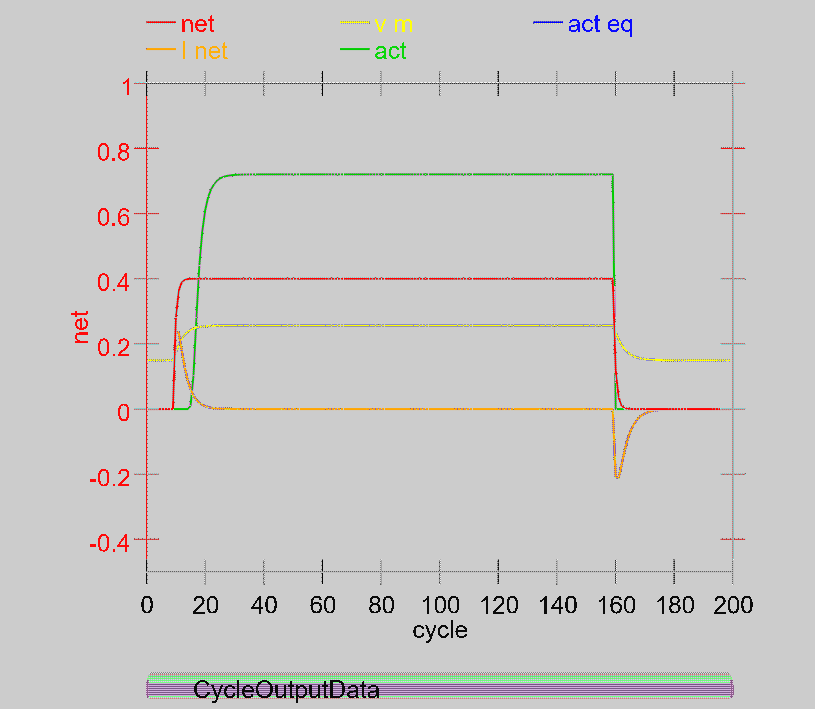
\includegraphics[scale=0.3]{Media/Main/EQ1/2.4.S0G.png}
\caption{Graphical output data of \cref{Q4.1} when running a value of 0.15 for $e_{rev\_l}$.}
\label{Q4.4}
\end{figure}

\begin{figure}[H]
\centering
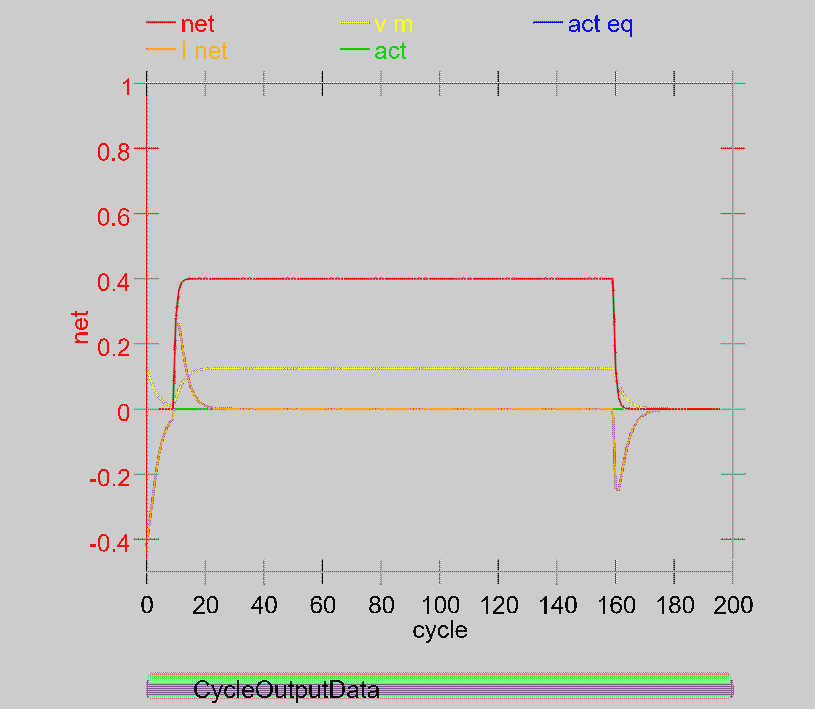
\includegraphics[scale=0.3]{Media/Main/EQ1/2.4.S1G.png}
\caption{Graphical output data of \cref{Q4.2} when running a value of 0.0 for $e_{rev\_l}$.}
\label{Q4.5}
\end{figure}

\begin{figure}[H]
\centering
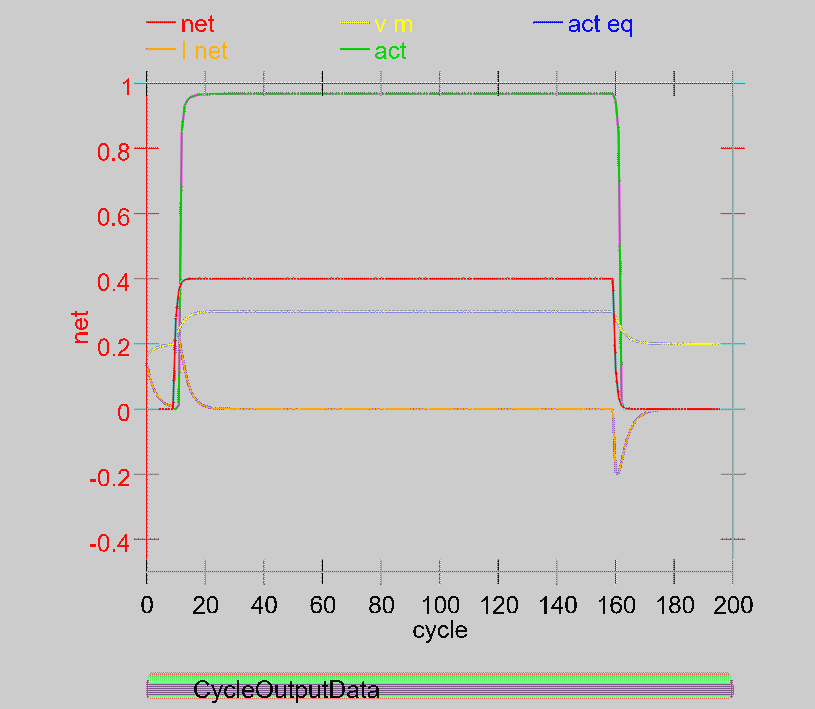
\includegraphics[scale=0.3]{Media/Main/EQ1/2.4.S2G.png}
\caption{Graphical output data of \cref{Q4.3} when running a value of 0.2 for $e_{rev\_l}$.}
\label{Q4.6}
\end{figure}
\end{multicols}

\subsubsection{Task 2.5}
\label{Q1:Expl 2.6.1(2.5) SubSubSection}

\begin{tcolorbox}[colback=gray!20!white,colframe=gray!20!white]
  \emph{\textbf{Question 2.5 (a)} What happens to the unit’s activity if you change the excitatory reversal potential $e_{rev\_e}$ from 1 to .5? Why does this happen? \textbf{(b)} Can you com- pensate for this by changing the value of $g_{bar\_e}$? To two decimal places, use the simulator to find the value of $g_{bar\_e}$ that gives essentially the same activation value as the default parameters. \textbf{(c)} Then use the same approach as in question 2.2 to solve for the exact value of $g_{bar\_e}$ that will compensate for this change in $e_{rev\_e}$ (use .256 for the membrane potential under the default parameters, and show your math). [Mark: 10]}
\end{tcolorbox} 
\vspace{0.5cm}

By changing the excitatory reversal potential $e_{rev\_e}$ value from 1.0 to 0.5 as seen in \cref{Q5.4}, the activation value is zero this is because the excitatory reversal potential must equal to 1 for any response in the activation level as the $g_{bar\_e}$ is at 0.4. The defaults parameters gave an activation level of 0.204, in \cref{Q5.5} where the value of $g_{bar\_e}$ is 1.22 which gives an activation level of 0.7191, this is the closest to the activation level to two decimal places. \\

\newpage
\begin{multicols}{2}
\begin{figure}[H]
\centering
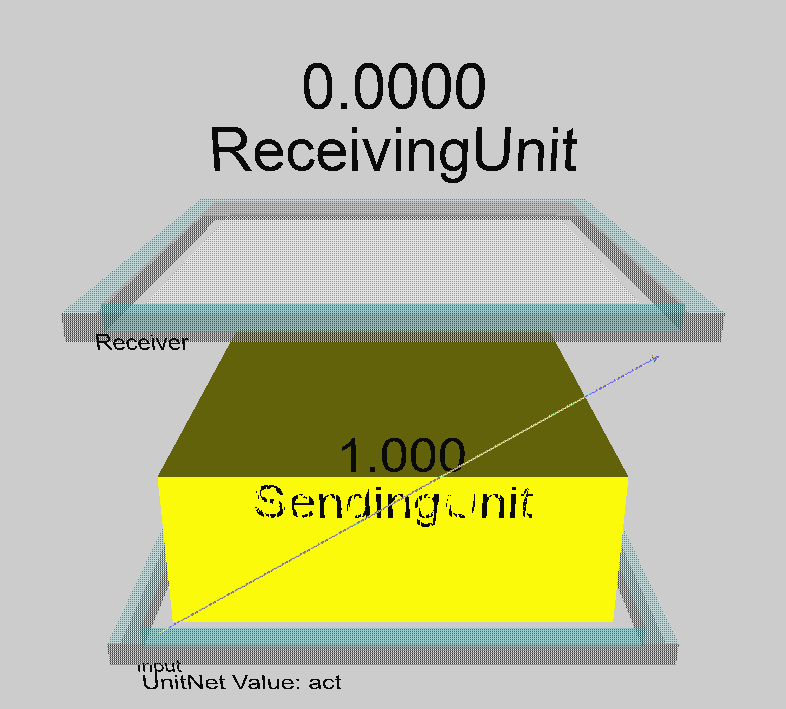
\includegraphics[scale=0.225]{Media/Main/EQ1/2.5.S1.png}
\caption{Visual representation of the sending and receiving units with $g_{rev\_e}$ at a value of 0.4.}
\label{Q5.1}
\end{figure}

\begin{figure}[H]
\centering
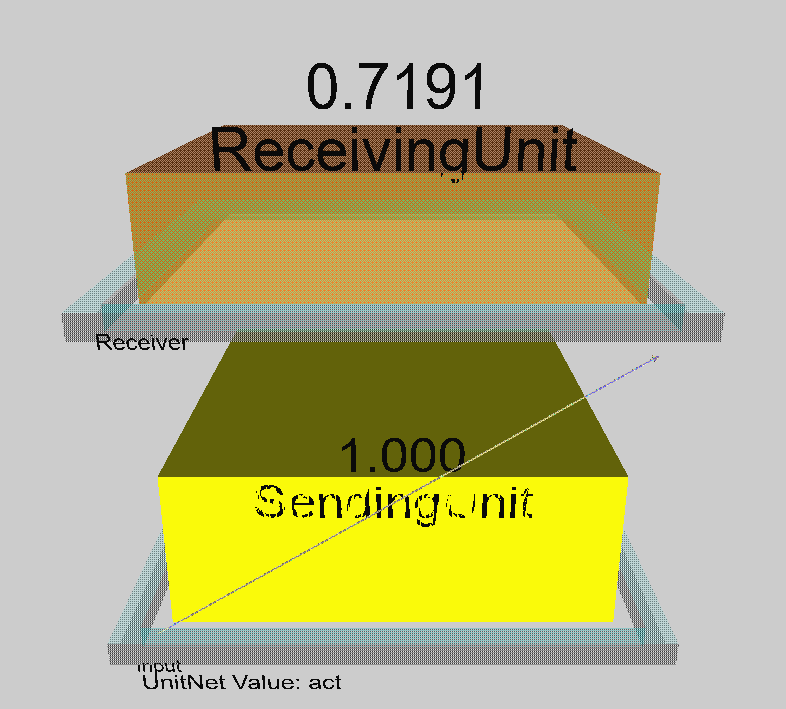
\includegraphics[scale=0.225]{Media/Main/EQ1/2.5.S2.png}
\caption{Visual representation of the sending and receiving units with $g_{rev\_e}$ at a value of 1.22.}
\label{Q5.2}
\end{figure}

\begin{figure}[H]
\centering
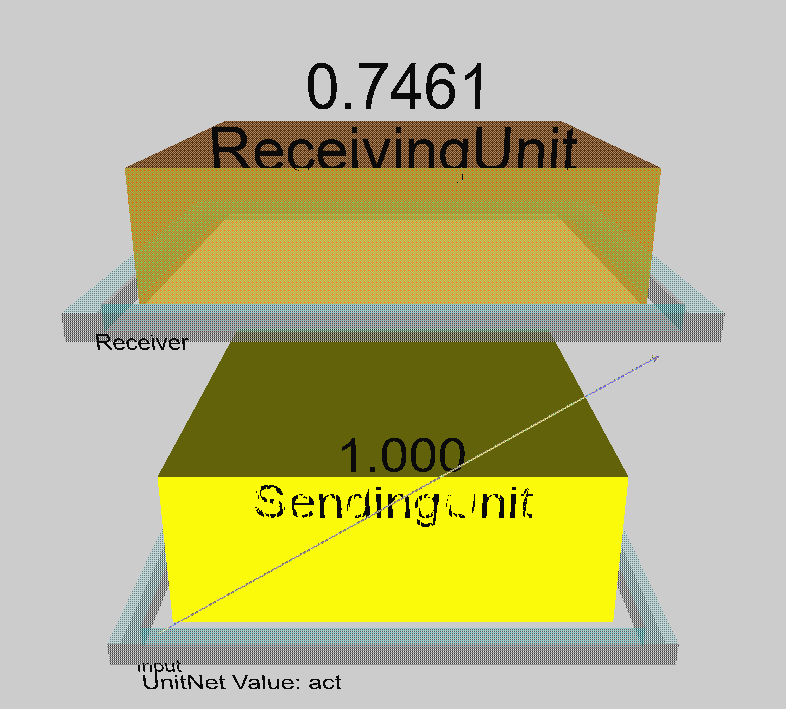
\includegraphics[scale=0.225]{Media/Main/EQ1/2.5.S3.png}
\caption{Visual representation of the sending and receiving units with $g_{rev\_e}$ at a value of 1.23.}
\label{Q5.3}
\end{figure}

\begin{figure}[H]
\centering
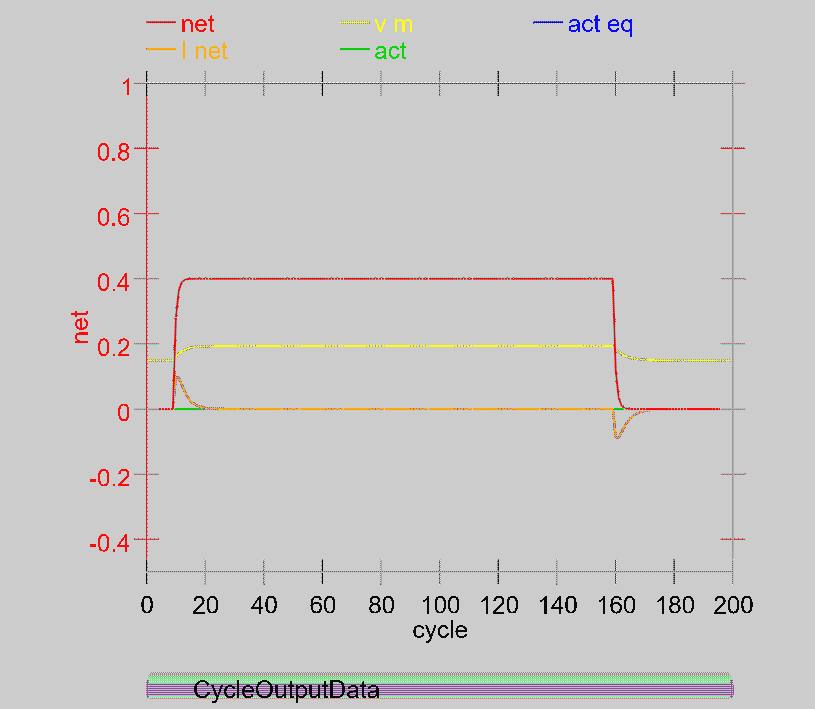
\includegraphics[scale=0.3]{Media/Main/EQ1/2.5.S1G.png}
\caption{Graphical output data of \cref{Q5.1} when running a value of 0.4 for $g_{rev\_e}$.}
\label{Q5.4}
\end{figure}

\begin{figure}[H]
\centering
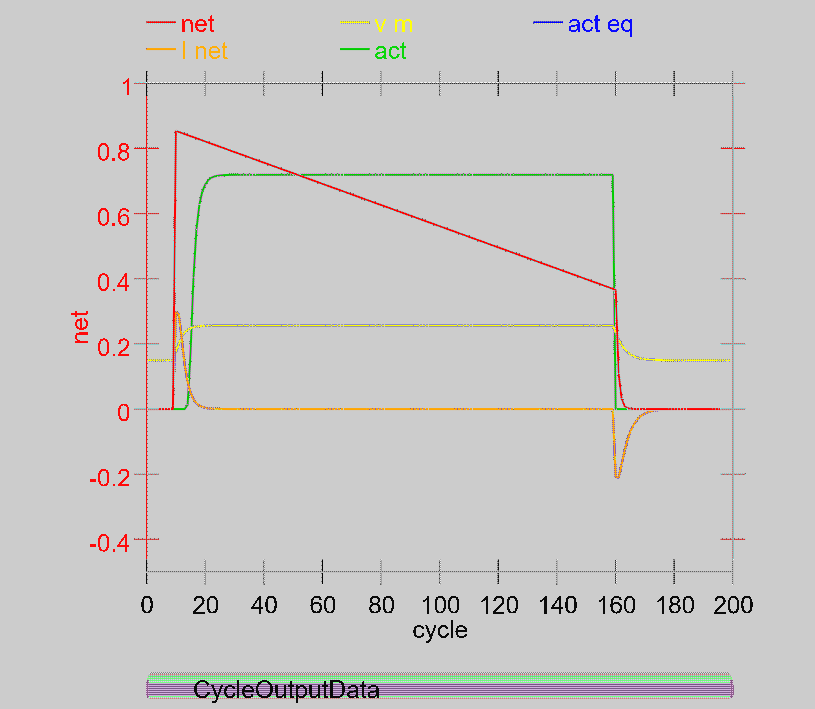
\includegraphics[scale=0.3]{Media/Main/EQ1/2.5.S2G.png}
\caption{Graphical output data of \cref{Q5.2} when running a value of 1.22 for $g_{rev\_e}$.}
\label{Q5.5}
\end{figure}

\begin{figure}[H]
\centering
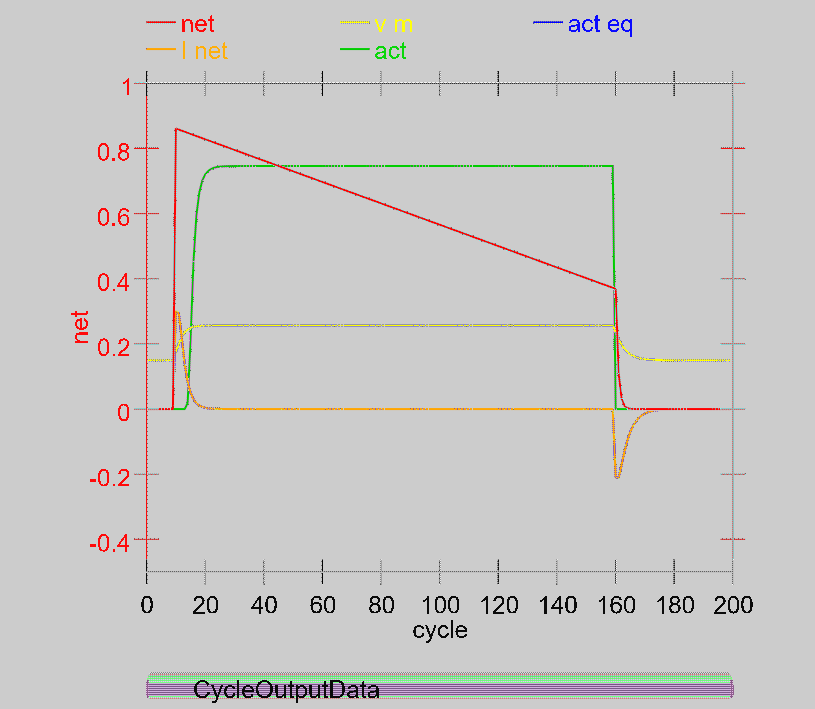
\includegraphics[scale=0.3]{Media/Main/EQ1/2.5.S3G.png}
\caption{Graphical output data of \cref{Q5.3} when running a value of 1.23 for $g_{rev\_e}$.}
\label{Q5.6}
\end{figure}
\end{multicols}